% !TeX program = xelatex
% ↑ Automatische Auswahl für XeLaTeX compiler

% Das ist mein Template für die TX000 Arbeiten. Nicht perfekt, also falls ihr Verbesserungsvorschläge habt, stellt gerne einen Pull-Request. https://github.com/NikomitK/TX000_Template
% Bitte lasst auch einen star auf github da, danke.
% Wenn ihr die cite funktion von LaTeX nutzen wollt, müsst ihr einfach die Quellen im bibtex Format in die sources.bib datei kopieren, google scholar z.B. hat bei den Quellen einen Button mit dem man das so bekommt, auch viele andere websites.
% Bilder kommen in den images Ordner, den müsst ihr beim abrufen eines Bildes nicht angeben, passiert automatisch.


% Trag hier deine Daten ein, die entsprechenden Felder werden automatisch angepasst.
\def\meinTitel{Title}
\def\artDerArbeit{STUDIENARBEIT}
\def\meinName{Ralf Kunath}
\def\meinKurs{TINF22F}
\def\meineMatrikelNr{Matrikelnummer}
\def\firmenName{Unternehmens-Name}
\def\abteilungsName{Abteilungsname}
\def\projektBetreuer{Vorname Nachname}
\def\ausbildungsLeiter{Vorname Nachname}
\def\abgabeDatum{dd.MM.yyyy}
%-----------------------------------------------------------------------------------


\documentclass[12pt]{report}
\usepackage[heightrounded]{geometry}
\geometry{
	a4paper,
	lmargin=3.1cm, %Seitenrand left
	tmargin=2.8cm, %Seitenrad top
	headsep=35pt %Abstand von Kopfzeile
}
\usepackage{amsmath}
\usepackage[utf8]{inputenc}
\usepackage{enumitem}
\usepackage{hyperref}
\usepackage[onehalfspacing]{setspace}
\usepackage[compact]{titlesec}
\usepackage{cite} % Zitierungen
\usepackage{struktex} % Struktogramme
\usepackage{array} % kp hat chatgpt benutzt
\usepackage{longtable} % Tabelle über einen seitenumbruch
\usepackage[nohyperlinks, printonlyused]{acronym} % abkürzungsverzeichnis
\usepackage{fontspec}
\usepackage{blindtext} % LoremIpsum
\usepackage{fancyhdr} % Kopf- und Fußzeile
\usepackage[export]{adjustbox} % Bilder alignment
\usepackage{stfloats} % Tabular at bottom
%\usepackage[table]{xcolor} %Tabellen farben
\usepackage{tabularx} % Anpassbarere tabellen
\usepackage{easyreview} % Review anmerkungen

\usepackage[utf8]{inputenc} % this is needed for umlauts
\usepackage[ngerman]{babel} % this is needed for umlauts
\usepackage[T1]{fontenc}    % this is needed for correct output of umlauts in pdf


\usepackage{subcaption} % Für subfigures glaub


\usepackage{tikz} % Zum zeichnen
\usetikzlibrary{calc}
\usetikzlibrary{shapes.geometric, arrows}
\setmainfont[Scale=1.1]{Arial}

%--------------------Flowcharts--------------------
\tikzstyle{startstop} = [rectangle, rounded corners, minimum width=3cm, minimum height=1cm,text centered, draw=black, fill=red!30]
\tikzstyle{io} = [trapezium, trapezium left angle=70, trapezium right angle=110, minimum width=3cm, minimum height=1cm, text centered, draw=black, fill=blue!30]
\tikzstyle{process} = [rectangle, minimum width=3cm, minimum height=1cm, text centered, draw=black, fill=orange!30]
\tikzstyle{decision} = [diamond, minimum width=3cm, minimum height=1cm, text centered, draw=black, fill=green!30]
\tikzstyle{arrow} = [thick,->,>=stealth]
%--------------------------------------------------


%--------------------Codeblöcke--------------------
\usepackage{listings} %Für Codeblöcke
\usepackage{color} %Farben für Codeblöcke?
\definecolor{dkgreen}{rgb}{0,0.6,0}
\definecolor{gray}{rgb}{0.5,0.5,0.5}
\definecolor{mauve}{rgb}{0.58,0,0.82}

\lstset{
	language=Java,
	aboveskip=3mm,
	belowskip=3mm,
	showstringspaces=false,
	columns=flexible,
	basicstyle={\small\ttfamily},
	numbers=none,
	numberstyle=\tiny\color{gray},
	keywordstyle=\color{blue},
	commentstyle=\color{dkgreen},
	stringstyle=\color{mauve},
	breaklines=true,
	breakatwhitespace=true,
	tabsize=3
}
%-------------------------------------------------

\usepackage{graphicx} %Package für Bilder
\graphicspath{ {./images/} } %Ordner für Bilder

\sloppy % damit lange Wörter nicht über die Zeile hinausgeschrieben werden.

%--------------------Chapter Heading--------------------
\makeatletter
\def\@makechapterhead#1{%
	\vspace*{-20\p@}%
	{\parindent \z@ \raggedright \normalfont
		\ifnum \c@secnumdepth >\m@ne
		%\huge\bfseries \@chapapp\space \thechapter
		\Huge\bfseries \thechapter.\space%
		%\par\nobreak
		%\vskip 20\p@
		\fi
		\interlinepenalty\@M
		\Huge \bfseries #1\par\nobreak
		\vskip 20\p@
}}
\makeatother
\makeatletter
\def\@makeschapterhead#1{%
	\vspace*{-20\p@}%
	{\parindent \z@ \raggedright \normalfont
		%\huge\bfseries \@chapapp\space \thechapter
		\Huge\bfseries\space%
		%\par\nobreak
		%\vskip 20\p@
		\interlinepenalty\@M
		\Huge \bfseries #1\par\nobreak
		\vskip 20\p@
}}
\makeatother
%-------------------------------------------------------

%\addto\captionsngerman{\renewcommand{\listfigurename}{}}
 % titel von abbildungsverzeichnis weg?

\setlength\parindent{0pt} %Auto Einrücken deaktivieren


%-------------Setup für Inhaltsverzeichnis--------------
\renewcommand{\contentsname}{Inhaltsverzeichnis} %Umbenennung TOC

\usepackage{tocloft} % Formatierung TOX

\setlength{\cftbeforetoctitleskip}{0pt}

\setlength{\cftsubsecnumwidth}{4em} %abstand kapitelnummer - titel

\renewcommand{\cfttoctitlefont}{\huge\bfseries}
\renewcommand{\cftloftitlefont}{\huge\bfseries}

\renewcommand\cftchapfont{\Large\bfseries}
\renewcommand\cftchappagefont{\large}

\renewcommand\cftsecfont{\large\bfseries}
\renewcommand\cftsecpagefont{\large}

\renewcommand\cftsubsecfont{\large}
\renewcommand\cftsubsecpagefont{\large}

\renewcommand\cftsubsubsecfont{\normalsize}
\renewcommand\cftsubsubsecpagefont{\normalsize}


\renewcommand\cftchapafterpnum{\par\addvspace{8pt}}
\renewcommand\cftsecafterpnum{\par\addvspace{8pt}}
\renewcommand\cftsubsecafterpnum{\par\addvspace{6pt}}
\renewcommand\cftsubsubsecafterpnum{\par\addvspace{6pt}}
%-------------------------------------------------------


%------------------Setup für LoF/LoT--------------------
\makeatletter
\renewcommand{\@cftmakeloftitle}{}
\renewcommand{\@cftmakelottitle}{}
\makeatother
\setlength{\cftfigindent}{0em} % change indentation of e.g. "Figure 1" within list of figures
\renewcommand\cftfigfont{\large}
\renewcommand\cftfigpagefont{\large}
\setlength{\cfttabindent}{0em} % change indentation of e.g. "Figure 1" within list of figures
\renewcommand\cfttabfont{\large}
\renewcommand\cfttabpagefont{\large}
\setlength{\cftbeforeloftitleskip}{0pt}
\setlength{\cftbeforelottitleskip}{0pt}
%-------------------------------------------------------


%----------------Setup für Verlinkungen-----------------
\usepackage{hyperref}
\hypersetup{
	colorlinks,
	citecolor=black,
	filecolor=black,
	linkcolor=black,
	urlcolor=black
}
%-------------------------------------------------------


%-------------Kopf-/Fußzeile für Titlepage--------------
\fancypagestyle{titlepage}
{
	\fancyhead[L]{
\includegraphics[scale=0.09]{firmenlogo}}
	\fancyhead[R]{
\includegraphics[scale=0.25]{dhbw}}
	\renewcommand{\headrulewidth}{0pt}
	\fancyfoot[C]{}
}
%-------------------------------------------------------

\begin{document} 
	
	\begin{titlepage}
		\thispagestyle{titlepage}
		\newcommand\HRule{\rule{\textwidth}{1pt}} %Titellinien

		
		\begin{center}
			
			\vspace*{2cm}
			
			%Title
			\begin{spacing}{2}
				{ \huge \bfseries \MakeUppercase{\meinTitel}}
				%{ \large \bfseries subTitle}\\[0.4cm]
			\end{spacing}
			
			\vspace*{1.5cm}
			
			%Art der Arbeit
			\Large \artDerArbeit
			
			\vspace*{3cm}
			
			%Hochschule
			{\LARGE Studiengang Informatik}\\
			{\LARGE an der Dualen Hochschule}\\
			{\LARGE Baden-Württemberg Stuttgart}\\

			\vspace*{2.5cm}
			
			\Large von \meinName
			
			\vspace*{1.5cm}
			
			\Large Abgabedatum: \abgabeDatum
			

			\begin{table*}[bp]
				\begin{tabular}{l l l l}
					Kurs: & \meinKurs & Matrikelnummer: & \meineMatrikelNr  \\
					Unternehmen: & \firmenName & Ausbildungsleiter: & \ausbildungsLeiter\\
					Abteilung: &  \abteilungsName & Projektbetreuer: &  \projektBetreuer\\
				\end{tabular}
			\end{table*}
			
			
		\end{center}
		
	\end{titlepage}


%------------------Kopf- und Fußzeile-------------------
\spacing{1.5}

\fancypagestyle{plain}{
	\fancyfoot[L]{\meinName\\
		 \meinKurs}
	\fancyfoot[C]{Seite \thepage\ }% von \pageref{LastPage}}
	\fancyfoot[R]{\abgabeDatum}
}

\pagestyle{plain}
\fancyhead{}


\fancyhead[L]{
\includegraphics[scale=0.09]{firmenlogo}}
\fancyhead[C]{\nouppercase\leftmark}
\fancyhead[R]{
\includegraphics[scale=0.25]{dhbw}}

\renewcommand{\footrulewidth}{0.4pt} %Linie für Fußzeile


\renewcommand{\sectionmark}[1]{\markboth{#1}{}} 
%-------------------------------------------------------

\pagenumbering{Roman}
\newpage
\chapter*{Abstract}
\addcontentsline{toc}{chapter}{\protect\numberline{}Abstract}
Hier kommt der Abstract.
\newpage

%------------------Inhaltsverzeichnis-------------------

\addcontentsline{toc}{chapter}{\protect\numberline{}Inhaltsverzeichnis}
\tableofcontents
\addtocontents{toc}{}
\thispagestyle{plain}
%-------------------------------------------------------


\newpage
\chapter*{Ehrenwörtliche Erklärung}
\addcontentsline{toc}{chapter}{\protect\numberline{}Ehrenwörtliche Erklärung}

Ich erkläre hiermit ehrenwörtlich, dass ich die vorliegende Arbeit selbstständig und ohne Benutzung anderer als der angegebenen Hilfsmittel angefertigt habe. Aus den benutzten Quellen, direkt oder indirekt, übernommene Gedanken habe ich als solche kenntlich gemacht.
\\
\\
\\
Diese Arbeit wurde bisher in gleicher oder ähnlicher Form oder auszugsweise noch keiner anderen Prüfungsbehörde vorgelegt und auch nicht veröffentlicht

\vspace{2.5cm}

\parbox{6.5cm}{\hrule\medskip Ort, Datum}  \hfill \parbox{6.5cm}{\hrule\medskip Unterschrift} \hspace{3cm}


%********************************
%Abbildungsverzeichnis
%********************************
\newpage
\chapter*{Abbildungsverzeichnis}
\addcontentsline{toc}{chapter}{\protect\numberline{}Abbildungsverzeichnis}

\listoffigures




%********************************
%Tabellenverzeichnis
%********************************
\newpage
\chapter*{Tabellenverzeichnis}
\addcontentsline{toc}{chapter}{\protect\numberline{}Tabellenverzeichnis}

\listoftables


\newpage
\chapter*{Abkürzungsverzeichnis}
\addcontentsline{toc}{chapter}{\protect\numberline{}Abkürzungsverzeichnis}
\markboth{Abkürzungsverzeichnis}{Abkürzungsverzeichnis} %Benötigt, damit das im header steht

%********************************
%Abkürzungsverzeichnis
%********************************
\begin{acronym}[SOAP]
	\acro{BA}{Beispiel Acronym}
\end{acronym}


%Speichern des page counters, um bei Literaturverzeichnis weiter zu zählen.
\newcounter{frontmatterPage}
\addtocounter{frontmatterPage}{\value{page}} 

\newpage
\pagenumbering{arabic}
\chapter{Einleitung}


%********************************
%Einleitung
%********************************
\chapter{Grundlagen}
\section{Instagram}
Instagram ist eine Social Media Plattform, welche darauf auf welcher Nutzer, Bilder und kurze Videos (Reels) teilen können. Die Plattform wird von vielen (oftmals jüngeren) Personen [Quelle] genutzt, um Erlebnisse, Meinungen, usw. mit anderen Menschen zu teilen. Dafür werden diese Bilder und Videos entweder als Post permanent hochgeladen, oder als Story nur für 24 Stunden. Ein solcher Account kann dabei entweder öffentlich oder privat gestellt werden, somit kann der Nutzer bestimmen, ob jeder Instagram-Nutzer oder nur die Follower des Accounts die Posts sehen können [Quelle]. 
Jeder Nutzer hat die Möglichkeit unter einem Post einen Kommentar zu verfassen, und somit zum Inhalt des Posts Stellung zu beziehen, ebenfalls ist es möglich Posts mit einem Like zu bewerten.
\newline

Neben den normalen privaten Nutzern, wird Instagram aber auch von vielen Influenzern, Politikern bzw. Parteien oder anderen politischen Gruppen, Unternehmen und Betrügern verwendet. So wird Instagram oft als Plattform zum verbreiten von Nachrichten über politischen, wirtschaftlichen oder gesellschaftlichen Ereignissen bzw. Themen verwendet[Quelle].
\newline


\section{TikTok}
\label{TikTokAllgemein}
TikTok ist ähnlich aufgebaut wie Instagram, allerdings konzentriert sich diese Plattform auf reine kurz Videos (2024 im schnitt 42.68 Sekunden [TikTok 1]). TikTok gilt dabei als die erste Plattform welche ein scrolling Prinzip eingeführt hat, was darauf basiert, dass das nächste Video angezeigt wird, sobald der Nutzer nach unten Scrollt [Quelle]. Genau wie bei Instagram wird auch hier mit Likes und Kommentaren gearbeitet.Auch auf TikTok wird von sowohl privaten Personen als auch Personen des öffentlichen Lebens genutzt, ähnlich wie Instagram.
\newline

Demographisch gesehen ist TikTok auf den Vormarsch, und genießt seit einigen Jahren einen rasanten Anstieg in der Beliebtheit.
Auch wenn dieser in den vergangenen Jahren etwas abgeflacht ist, wächst die Plattform auch jetzt noch schnell weiter [TikTok 2].
 
 
\begin{figure}[h]
	\centering
	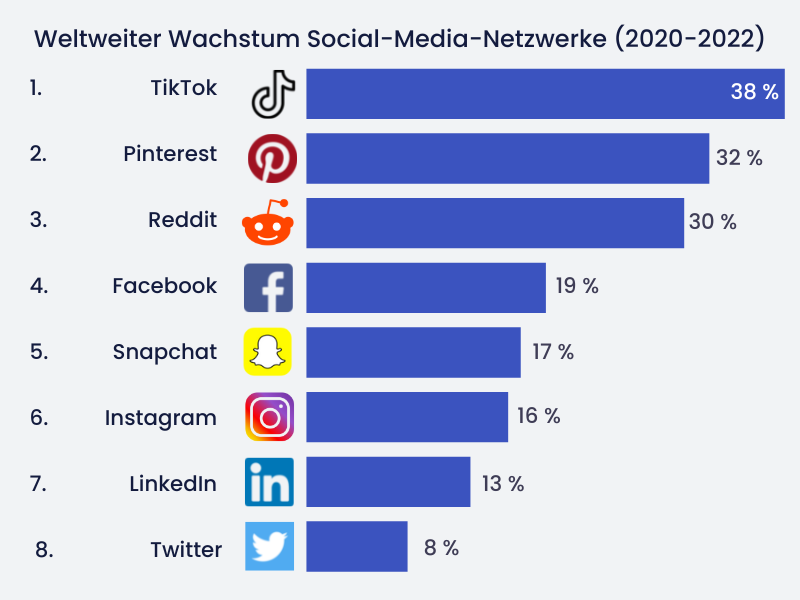
\includegraphics[width=0.7\textwidth]{../abbildungen/Social-Media-Wachtstum.png} 
	\caption{Wachstumsvergleich Social Media}
	\label{fig:WachstumsVergleich}
\end{figure}

Dieses starke Wachstum kann damit erklärt werden, dass das zentrale Feature von TikTok, die kurz Videos, passen zur schnellen Natur der Sozialen Medien, viele Nutzer befassen sich nur ein paar Sekunden mit einem Post und geht dann zum nächsten Inhalt [TikTok 3].
\newline





\section{Algorithmus}
Sowohl Instagram wie auch TikTok haben einen Algorithmus [Quelle], welcher die angezeigten Inhalte der Einzelnen Nutzer bestimmt. Der Algorithmus einer Plattform ist genauso wie ihr Prinzip ein wichtiger Faktor für den Erfolg, denn nur wenn die Nutzer Inhalte angezeigt bekommen, welche sie interessieren, hat die App auf langfristig Erfolg [Quelle].
\newline

Da der Algorithmus dementsprechend wichtig ist, ist dieser bei sowohl Instagram wie auch TikTok geheim [Quelle], und Faktoren welche Einfluss auf diesen haben können nur anhand von durchgeführten Test vermutet werden [Quelle].

\subsection{Instagram}
\label{AlgInsta}
Laut Wissenschaft.de sind die Schlüsselfaktoren für den Instagram Algorithmus sind die 
Interessen,
 dafür wird aus vergangenem Verhalten ermittelt ob der Nutzer Interesse an dem Thema hat:
\begin{itemize}
	\item \textbf{Beziehung}\\
	mit welchen Accounts der Nutzer häufig und lange interagiert.
	\item \textbf{Aktualität},\\
	wie aktuell (neu) der Post ist.
	\item \textbf{Frequenz}\\
	die Frequenz steht im Zusammenhang mit der Aktualität, es wird überprüft, wie oft der Nutzer Instagram benutzt, und dementsprechend wird die Aktualität angepasst (häufige Nutzung → neuere Posts, seltene Nutzung → auch ältere Posts).
	\item \textbf{Following}\\
	je nachdem, wie vielen und welchen Accounts der Nutzer folgt, werden die Inhalte angezeigt.
\end{itemize}


Instagram nutzt allerdings, laut der Quelle, nicht nur mit einem sondern mit drei Algorithmen, welche den Feed auf der Startseite, den Explorer Bereich und die Reels jeweils einen separaten Algorithmus [Algorythmus 1].

\subsection{TikTok}
\label{AlgTikTok}
Bei TikTok wird der Algorithmus, laut Content Managerin Simone Bogner, durch folgende Schlüsselfaktoren bestimmt:
\begin{itemize}
	\item \textbf{Wiedergabedauer}\\
	Wie lange wird ein Video angeschaut.
	\item \textbf{Engagement-Metriken},\\
	Wie oft wird ein Video geteilt, kommentiert geliked, etc.
	\item \textbf{Video-Informationen}\\
	Titel, Beschreibung etc. geben Informationen über den Inhalt eines Videos.
	\item \textbf{Frequenz}\\
	siehe \ref{AlgInsta}
	\item \textbf{Geräte und Kontoeinstellungen}\\
	Angaben wie Sprache, Herkunftsland, Alter, etc.
\end{itemize}

Der TikTok Algorithmus ist also sehr ähnlich wie der Instagram Algorithmus, wobei die genaue Gewichtung natürlich nicht bekannt ist. Auch ist es wahrscheinlich das bei beiden Angaben fehlen, welche von den jeweiligen Plattformanbietern geheim gehalten werden [Algorithmus 2]


\section{Datenschutzprobleme bei Instagram und TikTok}

Sowohl Instagram als auch TikTok sind aufgrund ihrer Datenschutzpraktiken in die Kritik geraten und wurden mit erheblichen Geldstrafen belegt.

\subsection{Instagram}
Im September 2022 verhängte die irische Datenschutzbehörde (Data Protection Commission, DPC) eine Geldstrafe von 405 Millionen Euro gegen Instagram. Der Grund dafür war der Umgang mit Daten von Kindern und Jugendlichen. Es wurde festgestellt, dass Instagram es Nutzern im Alter von 13 bis 17 Jahren ermöglichte, Geschäftskonten zu erstellen, wodurch ihre Telefonnummern und E-Mail-Adressen öffentlich einsehbar waren. Zudem wurden die Konten von Minderjährigen standardmäßig auf „öffentlich“ gesetzt, sodass ihre Inhalte für alle Nutzer sichtbar waren. Diese Praktiken stellten Verstöße gegen die EU-Datenschutzgrundverordnung (DSGVO) dar. Meta, die Muttergesellschaft von Instagram, erklärte, dass diese Einstellungen inzwischen aktualisiert wurden und dass Konten von Nutzern unter 18 Jahren nun standardmäßig auf „privat“ gesetzt sind. Dennoch kündigte Meta an, die Entscheidung der DPC anzufechten.  
(Quelle: \href{https://www.spiegel.de/netzwelt/netzpolitik/datenschutz-instagram-muss-in-irland-405-millionen-euro-strafe-zahlen-a-50fe2d10-c014-4a68-9cb8-b0b590d7cca5}{Spiegel Online})

\subsection{TikTok}
TikTok wurde ebenfalls wegen Datenschutzverstößen sanktioniert. Im September 2023 verhängte die irische Datenschutzbehörde eine Geldstrafe von 345 Millionen Euro gegen das Unternehmen. Die Untersuchung ergab, dass TikTok zwischen Juli 2020 und Dezember 2020 die Daten von minderjährigen Nutzern nicht ausreichend schützte. Kritisiert wurde unter anderem, dass die Konten von Nutzern unter 16 Jahren standardmäßig auf „öffentlich“ gesetzt waren und dass der Registrierungsprozess nicht transparent genug war, um sicherzustellen, dass Eltern oder Erziehungsberechtigte informiert wurden. TikTok hat seitdem Maßnahmen ergriffen, um die Privatsphäre von Jugendlichen besser zu schützen, einschließlich der Änderung der Standardeinstellungen für neue Nutzer unter 16 Jahren auf „privat“.  
(Quelle: \href{https://www.euractiv.de/section/innovation/news/irische-datenschutzbehoerde-verhaengt-405-millionen-euro-strafe-gegen-instagram/}{Euractiv})

Diese Fälle verdeutlichen die Herausforderungen, denen soziale Medien im Hinblick auf den Schutz der Daten junger Nutzer gegenüberstehen. Es zeigt sich die Notwendigkeit kontinuierlicher Überprüfungen und Anpassungen von Datenschutzrichtlinien, um den gesetzlichen Anforderungen gerecht zu werden und die Privatsphäre der Nutzer zu schützen.


\section{Einfluss von Social Media auf Meinungen}
Wie oben in den Kapiteln \ref{TikTokAllgemein} erwähnt wird Social Media auch als Plattform für Marken politische Inhalte oder Betrugsversuche genutzt. Da jeder auf sozialen Medien Posten kann, können so auch falsche oder Einseitige Informationen verbreitet werden [Quelle], was solchen Plattformen große Macht gibt, Beispiele hierzu sind der US-Wahlkampf oder das verbreiten von falsch-Informationen während der Corona-Pandemie [Quelle], sowie der Ukraine-Krieg und die kämpfe zwischen Israel und der Hamas.
\newline 

Laut einem Artikel der Medienanstallt NRW [Einfluss Social Media 1] bewirkt der sogenannte Illusory Truth Effect, dass Menschen Sachverhalte glauben, welche öfter wieder holt wurden. Dieser Effekt kann in Sozialen Medien leicht zum tragen kommen, da Nachrichten schnell sehr weit verbreitet und öfter gepostet werden können. Da solche Plattformen, wie in Kapitel \ref{AlgInsta} und \ref{AlgTikTok} beschrieben, Nutzern oft ähnliche Inhalte anzeigen, werden diesen oft mehrfach die gleichen Informationen angezeigt, ohne deren Korrektheit zu überprüfen oder Alternativen anzugeben. Das kann den Illostry Truth Effect herbei führen. Gleiches kann auch passieren, wenn Posts oft gliked werden, oder die Kommentare positiv sind. 

\section{Fake-Accounts und Bots}
Fake-Accounts sind Accounts, welche eine andere bzw. falsche Identität vorgeben. Dazu zählen zum Beispiel Accounts, welche sich als andere Person oder Einrichtung ausgeben, wie etwa eine prominente Person oder eine Partei. Dann wird im Namen dieser Person im Internet gehandelt \cite{akhtar2023false}. Das kann verschiedene Gründe haben, hier ein paar Beispiele:
\begin{itemize}
	\item \textbf{Eigenprofilierung }\\
	Der Ruf der vorgegebenen Person wird für eigene Zwecke ausgenutzt, wie etwa Werbung für Produkte, Dienstleistungen, etc. oder das Erhalten von Informationen oder Geld.
	\item \textbf{Manipulation und Meinungsbeeinflussung},\\
	Der Ruf einer Person wird ausgenutzt, um die Meinung von Menschen zu beeinflussen \cite{reuters2025merz}.
	\item \textbf{Schädigung des Rufes}\\
	Der Ruf der vorgegebenen Person soll geschädigt werden.
\end{itemize}

Zu unterscheiden sind dabei Fake-Accounts, welche eine reale Person nachstellen, und die Accounts, welche eine erfundene Person nachstellen. Fake-Accounts, die keine direkte Person nachstellen, werden oft als Bots erstellt.

Bots sind Accounts, die im Normalfall in einer großen Anzahl erstellt werden, jedoch nicht direkt von einer Person kontrolliert werden, sondern von einem Programm, welches eine bestimmte Aufgabe bekommt. So werden Bots zum Beispiel dafür verwendet, um Posts zu liken, kommentieren und/oder zu reposten.  

Die Erstellung von Fake-Accounts und Bots kann verschiedene Vorteile für die Urheber haben:

\begin{itemize}
	\item \textbf{Verbreitung von Desinformation}: Bots und Fake-Accounts werden genutzt, um gezielt falsche Informationen zu verbreiten und so die öffentliche Meinung zu manipulieren \cite{akhtar2023false}.
	\item \textbf{Politische Einflussnahme}: Durch koordinierte Bot-Netzwerke können politische Narrative verstärkt und Wahlen beeinflusst werden \cite{reuters2025merz}.
	\item \textbf{Wirtschaftliche Vorteile}: Im Influencer-Marketing können Fake-Follower und Bot-Interaktionen genutzt werden, um eine größere Reichweite vorzutäuschen und höhere Werbeeinnahmen zu erzielen.
	\item \textbf{Soziale Manipulation}: Bots können eingesetzt werden, um soziale Trends zu beeinflussen oder bestimmte Themen in den Vordergrund zu rücken.
\end{itemize}

Die Präsenz von Fake-Accounts und Bots stellt eine Herausforderung für die Integrität sozialer Netzwerke dar und erfordert kontinuierliche Anstrengungen zur Identifizierung und Bekämpfung solcher manipulativer Praktiken.


\section{Datenerhebung von Meta und TikTok}

In den vorangegangenen Kapiteln wurde bereits erwähnt, dass für den Betrieb von Social-Media-Plattformen viele Daten gesammelt werden, insbesondere um die zuvor beschriebenen Algorithmen zu betreiben. Hierzu werden Daten wie das Nutzungsverhalten getrackt und gespeichert. Doch nicht nur dafür sammeln die Plattformbetreiber Daten; auch zur gezielten Schaltung von Werbung wird das Nutzungsverhalten analysiert, um potenzielle Interessen abzuleiten \cite{zdnet2020}.

\subsection{Konkretisierung der gesammelten Daten}

Meta, zu dem unter anderem Instagram und Facebook gehören, erhebt eine Vielzahl von Datenkategorien. Dazu zählen:

\begin{itemize}
	\item \textbf{Profilinformationen}: Name, E-Mail-Adresse, Telefonnummer, Geburtsdatum.
	\item \textbf{Standortdaten}: Ermittlung des ungefähren Standorts anhand von IP-Adressen oder GPS-Daten.
	\item \textbf{Kontaktdaten}: Zugriff auf das Adressbuch des Nutzers, um Verbindungen zu Freunden herzustellen.
	\item \textbf{Nutzungsdaten}: Informationen darüber, welche Inhalte angesehen, geliked oder geteilt werden, sowie die Verweildauer auf bestimmten Beiträgen.
	\item \textbf{Gerätedaten}: Details zum verwendeten Gerät, wie Modell, Betriebssystem und Spracheinstellungen.
\end{itemize}

Eine Studie von Clario zeigt, dass Facebook mehr als 70\% aller verfügbaren Datenkategorien abdeckt, während Instagram auf über 50\% kommt \cite{zdnet2020}.

TikTok, betrieben von der Firma ByteDance, sammelt vergleichbare Daten. Laut der Datenschutzrichtlinie von TikTok werden unter anderem folgende Informationen erfasst:

\begin{itemize}
	\item \textbf{Profilinformationen}: E-Mail-Adresse, Telefonnummer, Geburtsdatum, Benutzername und Passwort.
	\item \textbf{Geteilte Inhalte}: Fotos, Videos, Audioaufnahmen, Livestreams, Kommentare und Hashtags.
	\item \textbf{Technische Daten}: Gerätemodell, Betriebssystem, IP-Adresse und Spracheinstellungen.
	\item \textbf{Nutzungsdaten}: Angesehene oder geteilte Inhalte, Suchverlauf, verwendete Hashtags sowie Zeitpunkt, Dauer und Häufigkeit der Nutzung.
	\item \textbf{Standortdaten}: Ungefährer Standort, ermittelt durch SIM-Karten und IP-Adressen.
\end{itemize}

Zusätzlich kann TikTok auf Inhalte der Zwischenablage zugreifen, wenn Nutzer Inhalte hochladen oder bearbeiten \cite{erecht24}.

\subsection{Vergleich der Datensammlungsmethoden von Meta und TikTok}

Während Meta sowohl auf plattformeigene Daten als auch auf Informationen von Drittanbietern zurückgreift, um detaillierte Nutzerprofile zu erstellen, zeigt TikTok ein ähnliches Verhalten. Eine Untersuchung von URL Genius ergab, dass TikTok während eines Besuchs 14 Netzwerkkontakte aufzeichnete, von denen 13 von Drittanbietern stammten \cite{wuv2022}. Dies deutet darauf hin, dass TikTok umfangreiche Daten an externe Partner weitergibt, während Meta einen Großteil der Daten für eigene Zwecke nutzt.


\chapter{Analyse der bestehenden Maßnahmen gegen Fake-Accounts}
\section{Maßnahmen von Instagram und TikTok}
\subsection{Instagram}

Instagram hat verschiedene Strategien implementiert, um gegen Fake-Accounts und Bots vorzugehen:

\begin{itemize}
	\item \textbf{Einsatz von maschinellem Lernen:} \\
	Instagram verwendet maschinelle Lernalgorithmen, um nicht authentische Aktivitäten zu identifizieren und zu entfernen. Diese Algorithmen erkennen Muster wie unnatürlich schnelle Interaktionen oder unrealistische Follower-Wachstumsraten \cite{instagram_authenticity_measures}.
	
	\item \textbf{Identitätsverifizierung:} \\
	Seit August 2020 fordert Instagram Nutzer auf, ihre Identität zu bestätigen, wenn verdächtige Aktivitäten festgestellt werden. Dies dient dazu, die Authentizität der Community zu gewährleisten \cite{instagram_authenticity_measures}.
	
	\item \textbf{Einschränkung von Drittanbieter-Apps:} \\
	Im November 2018 begann Instagram damit, nicht authentische "Gefällt mir"-Angaben, Follower und Kommentare zu entfernen, die durch Drittanbieter-Apps generiert wurden. Nutzer, die solche Apps verwenden, werden aufgefordert, ihr Passwort zu ändern, um den Zugriff dieser Apps zu unterbinden \cite{instagram_reducing_inauthentic_activity}.
	
	\item \textbf{Rechtliche Schritte gegen Missbrauch:} \\
	Im Februar 2025 leitete Meta, die Muttergesellschaft von Instagram, rechtliche Schritte gegen Personen ein, die unerlaubt Instagram-Benutzernamen verkauften und unbefugt Konten wiederherstellten. Diese Maßnahmen zielen darauf ab, den Schwarzmarkt für Instagram-Dienste zu bekämpfen \cite{meta_lawsuits_black_market}.
\end{itemize}

Trotz dieser Bemühungen bleibt die Anzahl der Fake-Accounts auf Instagram signifikant. Schätzungen zufolge sind etwa 95 Millionen Accounts, was ungefähr 10\% aller Instagram-Profile ausmacht, Fälschungen \cite{instagram_fake_accounts_statistics}.

\subsection{Zahlen zu Instagram}

Schätzungen zufolge sind etwa 95 Millionen Accounts auf Instagram Bots oder Fake-Accounts, was ungefähr 10\% aller Profile ausmacht \cite{ghost_data_2018}. Diese Fake-Accounts werden häufig genutzt, um die Follower-Zahlen von Nutzern künstlich zu erhöhen, wodurch eine größere Reichweite vorgetäuscht wird. Dies ist insbesondere für Influencer von Interesse, die durch höhere Follower-Zahlen mehr Geld für Produktplatzierungen und Werbung verlangen können \cite{futurezone_2018}.

\newpage

\subsection{TikTok}
\label{AnalyTikTok}
TikTok verwendet ein automatisiertes Moderationssystem, das Inhalte eigenständig entfernen oder zur manuellen Überprüfung an Moderatoren weiterleiten kann. Zusätzlich setzt die Plattform auf die Mithilfe der Nutzer, die verdächtige Accounts oder Inhalte melden können \cite{tiktok_moderation_system}.

Ähnlich wie bei Instagram sind detaillierte Informationen über den genauen Aufbau des TikTok-Algorithmus nicht öffentlich zugänglich. TikTok hat jedoch einige grundlegende Faktoren offengelegt, die das Empfehlungssystem beeinflussen. Dazu zählen:

\begin{itemize}
	\item \textbf{Nutzerinteraktionen:} \\
	Dies umfasst das Ansehen, Liken, Teilen und Kommentieren von Videos sowie das Folgen von Accounts. Diese Interaktionen geben Hinweise auf die Vorlieben der Nutzer und beeinflussen die Inhalte, die ihnen empfohlen werden \cite{tiktok_algorithm_explained}.
	
	\item \textbf{Videoinformationen:} \\
	Informationen wie Untertitel, Hashtags, Sounds und verwendete Effekte spielen eine Rolle bei der Kategorisierung und Empfehlung von Inhalten \cite{tiktok_algorithm_explained}.
	
	\item \textbf{Geräte- und Account-Einstellungen:} \\
	Einstellungen wie Sprache, Ländereinstellungen und Gerätetyp werden ebenfalls berücksichtigt, haben jedoch einen geringeren Einfluss auf die Empfehlungen im Vergleich zu den anderen Faktoren \cite{tiktok_algorithm_explained}.
\end{itemize}

Es ist wichtig zu beachten, dass TikTok kontinuierlich an der Verbesserung seines Moderationssystems arbeitet, um die Verbreitung von Fake-Accounts und Bots zu minimieren. Dennoch bleibt die genaue Funktionsweise des Algorithmus weitgehend vertraulich, um Missbrauch zu verhindern und die Integrität der Plattform zu schützen.

\subsection{Zahlen zu TikTok}
Laut TikTok selber wurden im zweiten Quartal in 2024 94\% allen traffics, welcher von Fake-Accounts und Bots unternommen wurde, von den in \ref{AnalyTikTok} beschrieben automatischen Systemen durchgeführt.
\newline 

Weiter behauptet TikTok selber die Erstellung von 700 Millionen Fake-Accounts verhindert zu haben, und 940 Millionen Millionen Videos von Fake-Accounts gelöscht zu haben. Weiter wurden, laut eigenen Angaben 36 Billionen likes von derartigen Accounts verhindert und mehr als 379 Millionen gelöscht. Auch sollen 15 Billionen Follow-Anfragen frühzeitig erkannt und weitere 207 Millionen im Nachhinein gelöscht worden sein [AnalyTikTok 2].
\newline

Diese Angaben wurden alle von TikTok selber veröffentlicht, dementsprechend ist deren Korrektheit schwer zu überprüfen. Weiter gibt es keine Verhältnis Größen zu vielen Angaben, dementsprechend ist nicht überprüfbar wie effektiv TikTok gegen die Aktivität von Fake-Accounts vorgeht.


\section{Weiteres Vorgehen}
Da es keine genaueren Informationen den Algorithmen für die Fake-Account Bekämpfung von Instagram und TikTok
gibt, sowie keine Zahlen über das bekämpfen solcher Fake-Accounts, kann hier keine Analyse über die Effektivität der Unternehmen im Kampf gegen Bots und Fake-Accounts gemacht werden. Deshalb werden hier zum Vergleich andere Ansätze zur Erkennung von Fake-Accounts und Bots herangezogen.




\section{Verschiedene Algorithmen zur Erkennung von Fake-Accounts}


\subsection{Methode 1}
Der Ansatz zur Erkennung von Fake-Accounts basiert auf einem mehrstufigen Verfahren: Zunächst werden öffentliche Instagram-Profile automatisiert gesammelt und die enthaltenen Daten bereinigt. Anschließend werden aus diesen Daten relevante Merkmale extrahiert, die typische Verhaltensmuster von Accounts widerspiegeln. Mithilfe maschineller Lernverfahren wird ein Klassifikationsmodell trainiert, das zwischen authentischen und inauthentischen Profilen unterscheidet. Die kontinuierliche Evaluierung und der Einsatz des Modells im Echtbetrieb ermöglichen eine zuverlässige Identifikation von Fake-Accounts.
\newline

Besonders zwei Merkmale stehen dabei im Fokus:

\begin{itemize}[noitemsep, leftmargin=*, labelsep=1em]
	\item \textbf{Follower-Following-Ratio:} Fake-Accounts folgen oft vielen Nutzern, erhalten aber nur wenige Follower zurück. Ein hoher Unterschied zwischen Followings und Followern kann auf ein nicht authentisches Profil hinweisen. Um Anomalien zu erkennen, werden statistische Verfahren wie die Z-Score-Normalisierung eingesetzt. Dabei wird der Abstand zur Durchschnittsverteilung der Follow-Ratios berechnet und auffällige Profile als potenzielle Fake-Accounts markiert.
	
	
	\item \textbf{Interaktionsmuster und Engagement-Rate:} Fake-Accounts weisen oft eine niedrige Engagement-Rate auf, da sie wenige echte Interaktionen erhalten. Die Engagement-Rate wird durch die Formel \(\frac{\text{Anzahl der Interaktionen}}{\text{Anzahl der Follower}}\) berechnet. Um festzustellen, ob ein Account verdächtig ist, werden historische Interaktionsmuster analysiert und mit typischen Verhaltensweisen echter Nutzer verglichen. Besonders Accounts mit hohem Posting-Volumen, aber wenig bis keinen Kommentaren oder Likes, werden genauer untersucht.
\end{itemize}

\textbf{Implementierung:} Die Merkmalsextraktion erfolgt durch automatisiertes Scraping und API-Abfragen, wobei die gesammelten Daten standardisiert und in numerische Werte überführt werden. Vor dem Training werden die Daten bereinigt, normalisiert und fehlende Werte behandelt, um eine konsistente Analyse zu gewährleisten. 

Zur Klassifikation der Accounts wird der \textbf{Random Forest Algorithmus} verwendet. Dieser besteht aus einer Vielzahl von Entscheidungsbäumen, die jeweils auf unterschiedlichen Teilmengen der Trainingsdaten basieren. Jeder Baum trifft eine eigene Klassifikationsentscheidung, und das finale Ergebnis wird durch Mehrheitsentscheidung aggregiert.

\textbf{Optimierung des Algorithmus:} Zur Verbesserung der Modellleistung werden verschiedene Hyperparameter optimiert, darunter:

\begin{itemize}[noitemsep, leftmargin=*, labelsep=1em]
	\item Anzahl der Bäume im Wald (\textit{n\_estimators})
	\item Maximale Tiefe der Entscheidungsbäume (\textit{max\_depth})
	\item Mindestanzahl an Samples pro Blatt (\textit{min\_samples\_leaf})
	\item Verwendete Merkmale pro Split (\textit{max\_features})
\end{itemize}

Zur Evaluierung der Modellleistung werden mehrere \textbf{Metriken} herangezogen:

\begin{itemize}[noitemsep, leftmargin=*, labelsep=1em]
	\item \textbf{Accuracy}: Der Anteil der korrekt klassifizierten Accounts.
	\item \textbf{Precision}: Der Anteil der tatsächlich gefälschten Accounts unter allen als Fake klassifizierten Profilen.
	\item \textbf{Recall}: Der Anteil der erkannten Fake-Accounts unter allen tatsächlich gefälschten Profilen.
	\item \textbf{F1-Score}: Das harmonische Mittel aus Precision und Recall zur Gesamtbewertung der Modellleistung.
\end{itemize}

Die finale Modellbewertung erfolgt durch eine \textbf{Kreuzvalidierung}, bei der der Datensatz in mehrere Teilmengen unterteilt wird. Das Modell wird mehrfach auf verschiedenen Kombinationen aus Trainings- und Testdaten evaluiert, um eine stabile und verlässliche Leistungsbewertung zu gewährleisten.

Nach der Validierung wird das trainierte Modell in eine Echtzeit-Erkennungs-Pipeline integriert, um kontinuierlich neu erstellte oder verdächtige Profile zu analysieren. Durch diese automatisierte Überwachung können Fake-Accounts effizient identifiziert und entfernt werden. [Methode 1]

\section{Methode 2}

Die Identifikation von Fake-Accounts auf TikTok basiert auf einem mehrstufigen, datengetriebenen Ansatz, der sowohl regelbasierte Methoden als auch maschinelles Lernen kombiniert. Im Gegensatz zu allgemeinen Fake-Account-Detektionsverfahren wird hier insbesondere auf TikTok-spezifische Charakteristika eingegangen. Die Methode stützt sich primär auf zwei Kernansätze: (1) Analyse von Nutzerverhalten und (2) Erkennung von Anomalien durch Deep Learning.

\subsubsection{1. Analyse von Nutzerverhalten}

Der erste Ansatz konzentriert sich auf die Identifikation verdächtiger Interaktionsmuster, indem verschiedene Metriken untersucht werden, die für normale Nutzer untypisch sind. Dazu gehören:
\begin{itemize}
	\item \textbf{Follower-Following-Ratio:} Ein extrem hohes oder niedriges Verhältnis zwischen der Anzahl an Followern und den gefolgten Accounts kann ein Indikator für automatisierte Profile sein.
	\item \textbf{Interaktionsrate:} Das Verhältnis von Likes, Kommentaren und Shares zur Gesamtanzahl der Follower gibt Aufschluss über organische oder künstlich generierte Engagements.
	\item \textbf{Post-Frequenz:} Accounts, die innerhalb kurzer Zeit sehr viele oder extrem wenige Videos hochladen, können Anomalien aufweisen.
	\item \textbf{Hashtag-Nutzung:} Fake-Accounts nutzen oft bestimmte Hashtags übermäßig, um Reichweite zu generieren oder sich an Trends zu heften.
	\item \textbf{Video-Muster:} Wiederverwendung identischer oder leicht veränderter Inhalte kann auf automatisierte Generierung hindeuten.
\end{itemize}

Zur Verarbeitung dieser Metriken werden Entscheidungsbäume eingesetzt, die eine Regelbasis für verdächtige Verhaltensmuster erstellen. Dabei wird eine \textbf{Threshold-Analyse} durchgeführt, um Grenzwerte für auffällige Wertebereiche zu bestimmen. Diese Methode eignet sich besonders für Echtzeit-Analysen und ermöglicht eine schnelle erste Kategorisierung von verdächtigen Profilen.

\subsubsection{2. Erkennung von Anomalien durch Deep Learning}

Neben regelbasierten Methoden wird ein neuronales Netz trainiert, um komplexe Muster in Fake-Account-Verhalten zu erkennen. Hier kommt insbesondere ein \textbf{Convolutional Neural Network (CNN)} zum Einsatz, das auf TikTok-spezifische Merkmale optimiert ist. Folgende Aspekte werden berücksichtigt:
\begin{itemize}
	\item \textbf{Textuelle Merkmale:} Die Beschreibung von Videos, Biografien und Kommentaren werden mittels \textit{Natural Language Processing (NLP)} analysiert, um Sprachmuster und Spam-ähnliche Inhalte zu identifizieren.
	\item \textbf{Visuelle Erkennung:} Wiederverwendete oder KI-generierte Inhalte werden durch Bildähnlichkeitsanalysen erkannt, um massenhaft erstellte Fake-Videos zu identifizieren.
	\item \textbf{Zeitliche Muster:} Ein Long Short-Term Memory (LSTM)-Netzwerk analysiert die Aktivitätsmuster über einen längeren Zeitraum, um auffällige Veränderungen im Nutzungsverhalten zu erkennen.
\end{itemize}

Die Kombination aus CNN und LSTM ermöglicht eine detaillierte Analyse, die über einfache Regelwerke hinausgeht. Besonders durch den Einsatz von Transformer-Modellen können Fake-Accounts identifiziert werden, die sich adaptiv an Veränderungen in der Plattform anpassen.

\subsubsection{Modelltraining und Evaluation}

Zur Optimierung des Modells erfolgt eine \textbf{Feature Selection} mittels \textit{Principal Component Analysis (PCA)}, um irrelevante Datenpunkte zu eliminieren. Anschließend wird das Modell mit folgenden Metriken bewertet:
\begin{itemize}
	\item \textbf{Precision:} Gibt an, wie viele der als Fake klassifizierten Accounts tatsächlich gefälscht sind.
	\item \textbf{Recall:} Zeigt, wie viele der existierenden Fake-Accounts korrekt erkannt wurden.
	\item \textbf{F1-Score:} Harmonisches Mittel aus Precision und Recall zur Gesamtbewertung.
	\item \textbf{False Positive Rate:} Identifiziert, wie oft legitime Accounts fälschlicherweise als Fake eingestuft werden.
\end{itemize}

Die finale Implementierung erfolgt durch eine \textbf{Echtzeit-Analyse-Pipeline}, die kontinuierlich neue Fake-Account-Muster erkennt und die Modelle durch \textit{Online Learning} automatisch anpasst. Dadurch wird sichergestellt, dass das System gegen sich entwickelnde Fake-Account-Strategien robust bleibt.

[Methode 2]

\subsection{Vergleich der Methoden}

Die beiden Methoden zur Erkennung von Fake-Accounts auf Instagram und TikTok zeigen sowohl methodische Gemeinsamkeiten als auch wesentliche Unterschiede in der Herangehensweise. Während beide Verfahren auf der Extraktion relevanter Merkmale und der Nutzung maschineller Lernmodelle basieren, unterscheiden sie sich insbesondere in der Art der eingesetzten Algorithmen, der Datengrundlage sowie der Echtzeit-Implementierung.

\subsubsection{Gemeinsamkeiten}

Beide Ansätze folgen einer mehrstufigen Pipeline zur Identifikation verdächtiger Accounts, die sich in folgende zentrale Schritte gliedert:

\begin{itemize}
	\item \textbf{Automatisierte Datensammlung:} Beide Methoden sammeln öffentliche Profile der jeweiligen Plattform (Instagram bzw. TikTok) und bereinigen die extrahierten Daten.
	\item \textbf{Merkmalsextraktion:} Relevante Kennwerte wie Follower-Following-Ratio, Interaktionsrate und Post-Frequenz werden extrahiert, um charakteristische Muster von Fake-Accounts zu identifizieren.
	\item \textbf{Einsatz maschinellen Lernens:} Beide Verfahren setzen maschinelle Lernmodelle zur Klassifikation von Fake-Accounts ein.
	\item \textbf{Evaluierung der Modellleistung:} Accuracy, Precision, Recall und der F1-Score werden zur Messung der Klassifikationsgenauigkeit verwendet.
	\item \textbf{Echtzeit-Anwendung:} Die trainierten Modelle werden in eine Echtzeit-Überwachungs-Pipeline integriert, um kontinuierlich neue oder verdächtige Profile zu identifizieren.
\end{itemize}

\subsubsection{Unterschiede und vertiefte Analyse}

Trotz der gemeinsamen Grundstruktur gibt es signifikante Unterschiede zwischen den beiden Methoden, insbesondere in Bezug auf die eingesetzten Modelle, die Merkmalsselektion und die Echtzeitverarbeitung.

\textbf{1. Plattformabhängigkeit und Datenbasis}

Ein entscheidender Unterschied zwischen den Methoden liegt in der zugrunde liegenden Plattform:

\begin{itemize}
	\item \textbf{Methode 1 (Instagram):} Die Analyse konzentriert sich auf statische Profileigenschaften und Interaktionsmuster. Instagram-Accounts weisen oft ein klares Follower-Following-Muster auf, das durch den Random Forest Algorithmus effizient klassifiziert werden kann.
	\item \textbf{Methode 2 (TikTok):} Die hohe Dynamik der Plattform erfordert eine tiefergehende Analyse von Nutzerverhalten, Video-Inhalten und textbasierten Metadaten. Hier spielen neuronale Netzwerke eine entscheidende Rolle bei der Mustererkennung.
\end{itemize}

\textbf{2. Wahl des maschinellen Lernmodells}

Die Algorithmen zur Klassifikation der Fake-Accounts unterscheiden sich erheblich:

\begin{itemize}
	\item \textbf{Methode 1: Random Forest}
	\begin{itemize}
		\item Eignet sich gut für tabellarische Daten mit klar definierten Merkmalen.
		\item Bietet eine hohe Interpretierbarkeit und ermöglicht eine robuste Entscheidungsfindung durch Mehrheitsvoting.
		\item Zeigt Schwächen bei der Erkennung komplexer Muster und nichtlinearer Beziehungen.
	\end{itemize}
	
	\item \textbf{Methode 2: Deep Learning mit CNN und LSTM}
	\begin{itemize}
		\item CNNs sind besonders geeignet für die Analyse visueller Merkmale in TikTok-Videos, da sie Bildähnlichkeitsanalysen durchführen können.
		\item LSTM-Modelle ermöglichen eine zeitliche Betrachtung der Aktivitätsmuster, um ungewöhnliches Verhalten über einen längeren Zeitraum zu erfassen.
		\item Durch den Einsatz von Transformer-Modellen kann das System dynamisch auf veränderte Fake-Account-Strategien reagieren.
	\end{itemize}
\end{itemize}

\textbf{3. Merkmalsselektion und Reduktion}

Ein weiterer Unterschied liegt in der Vorverarbeitung und Auswahl der relevanten Merkmale:

\begin{itemize}
	\item \textbf{Methode 1:} Es erfolgt keine spezifische Merkmalsreduktion; die wichtigsten Features werden direkt durch den Random Forest Algorithmus gewichtet.
	\item \textbf{Methode 2:} Durch Principal Component Analysis (PCA) werden irrelevante Merkmale eliminiert, um die Rechenzeit zu optimieren und Overfitting zu vermeiden.
\end{itemize}

\textbf{4. Echtzeitüberwachung und Anpassungsfähigkeit}

Die Implementierung der Echtzeit-Überwachung unterscheidet sich stark:

\begin{itemize}
	\item \textbf{Methode 1:} Das Modell bleibt nach dem Training statisch und wird periodisch mit neuen Daten aktualisiert.
	\item \textbf{Methode 2:} Eine kontinuierliche Echtzeit-Anpassung mittels \textit{Online Learning} erlaubt die automatische Anpassung an neu auftretende Fake-Account-Muster, wodurch das System gegen adversariale Angriffe robuster bleibt.
\end{itemize}

\subsubsection{Zusammenfassung und Bewertung}

Methode 1 bietet eine robuste, interpretierbare Lösung für die Fake-Account-Detektion auf Instagram. Sie eignet sich besonders für Anwendungen, bei denen statische Merkmale eine hohe Aussagekraft besitzen und einfache, erklärbare Modelle bevorzugt werden. Allerdings stößt sie an Grenzen, wenn es um die Erkennung adaptiver Betrugsmethoden geht.

Methode 2 ist flexibler und leistungsfähiger in der Erkennung komplexer und dynamischer Muster. Der Einsatz von Deep Learning ermöglicht eine tiefere Analyse der Fake-Account-Aktivitäten auf TikTok, birgt jedoch höhere Anforderungen an Rechenleistung und Datenverfügbarkeit. Besonders die Integration von Transformer-Modellen zur kontinuierlichen Anpassung stellt einen entscheidenden Vorteil gegenüber der klassischen Herangehensweise dar.

Zusammenfassend lässt sich sagen, dass Methode 1 für einfache, interpretierbare Klassifikationsprobleme geeignet ist, während Methode 2 eine leistungsfähigere, aber auch komplexere Lösung darstellt, die sich dynamisch an neue Betrugsmuster anpassen kann.



\section{Weitere Methoden zur Erkennung von Fake-Accounts}

Zusätzlich zu den beschriebenen Methoden existieren weitere Ansätze, die sich mit der Identifikation von Fake-Accounts auf Instagram und TikTok befassen. Diese Methoden erweitern klassische Verfahren und nutzen moderne Techniken der Künstlichen Intelligenz und Graphenanalyse.

\subsection{Einsatz von Künstlicher Intelligenz (KI) zur Deepfake-Erkennung}
Mit der zunehmenden Verbreitung von KI-generierten Inhalten, insbesondere Deepfakes, ist die Identifizierung solcher manipulierten Medien essenziell. Spezialisierte KI-Modelle analysieren dabei subtile Unstimmigkeiten in Videos oder Bildern, wie unnatürliche Bewegungen oder inkonsistente Lichtverhältnisse, um gefälschte Inhalte zu erkennen. Dieser Ansatz ist besonders relevant, da auf Plattformen wie Instagram vermehrt KI-generierte Influencer auftauchen, die echte Modelle imitieren und deren Inhalte modifizieren \cite{wired2023deepfake}.

\subsection{2. Verhaltensbasierte Analyse durch Machine Learning}
Anstelle der ausschließlichen Betrachtung von Profilmerkmalen fokussiert sich dieser Ansatz auf das Verhalten von Accounts. Machine-Learning-Modelle werden trainiert, um Muster in der Interaktion eines Nutzers zu erkennen, wie z. B. die Frequenz und Art von Kommentaren, Likes oder Posts. Ungewöhnliche Aktivitätsmuster, die von typischem Nutzerverhalten abweichen, können auf automatisierte oder gefälschte Accounts hindeuten \cite{cresci2020decade}.

\subsection{Netzwerkbasierte Analyse}
Durch die Untersuchung der Verbindungen und Interaktionen zwischen verschiedenen Accounts können Cluster von Fake-Profilen identifiziert werden. Gefälschte Accounts neigen dazu, miteinander vernetzt zu sein oder ähnliche Follower-Strukturen aufzuweisen. Graphentheoretische Ansätze helfen dabei, solche Netzwerke zu visualisieren und Anomalien aufzudecken \cite{cao2020synthetic}.

\subsection{Nutzung von Butterfly AI für die Mustererkennung}
Butterfly AI ist ein Ansatz, der auf der Analyse von Datenströmen in Echtzeit basiert. Durch die kontinuierliche Überwachung von Aktivitäten auf Plattformen wie Instagram und TikTok kann Butterfly AI ungewöhnliche Muster oder plötzliche Veränderungen im Nutzerverhalten erkennen, die auf Fake-Accounts hindeuten könnten. Dieser proaktive Ansatz ermöglicht es, potenzielle Bedrohungen frühzeitig zu identifizieren und entsprechende Maßnahmen zu ergreifen \cite{stolfo2000behavior}.

Diese ergänzenden Methoden bieten erweiterte Perspektiven im Kampf gegen Fake-Accounts und tragen dazu bei, die Authentizität von Nutzern auf sozialen Plattformen sicherzustellen.

\section{Analyse der Kriterien}
\subsection{Kriterien aus behandelten Methoden}
\subsection{zusätzlich erarbeitete Kriterien}

%********************************
%Zusammenfassung und Ausblick
%********************************
\newpage
\chapter{Kritische Reflexion und Ausblick}
\blindtext


%********************************
%Literaturverzeichnis
%********************************
\newpage
\pagenumbering{Roman}
\setcounter{page}{\value{frontmatterPage}} %Bei \pagenumbering wird Seitenzähler zurückgesetzt, hier wird der gespeicherte Wert vom frontmatter weitergeführt
\addtocounter{page}{1}
\addcontentsline{toc}{chapter}{\protect\numberline{}Literaturverzeichnis}

%Quellenverzeichnis
\begin{thebibliography}{9}
	\bibitem{akhtar2023false}
	Author: Mohammad Majid Akhtar, Rahat Masood, Muhammad Ikram, Salil S. Kanhere, Release: 24.08.2023, Link:\url{https://arxiv.org/abs/2308.12497}, Used: 22.02.2025
	
	\bibitem{reuters2025merz}
	Author: Reuters, Release: 20.02.2025, Link:\url{https://www.reuters.com/world/europe/friedrich-merz-targeted-by-pro-russian-disinformation-before-german-vote-2025-02-20/}, Used: 22.02.2025
	
	\bibitem{tiktok2022}
	Author: Jana Wagner, Release: 14.02.2022, Link:\url{https://mads.de/die-psychologie-hinter-tiktok-was-macht-den-erfolg-der-app-aus/}, Used: 21.02.2025
	
	\bibitem{zdnet2020}
	Author: Stefan Beiersmann, Release: 03.11.2020, Link: \url{https://www.zdnet.de/88389353/studie-brandmarkt-facebook-instagram-und-tinder-als-groesste-datensammler}, Used: 22.02.2025
	
	\bibitem{erecht24}
	Author: eRecht24, Link: \url{https://www.e-recht24.de/datenschutz/13278-tiktok-datenschutz.html}, Used: 22.02.2025
	
	\bibitem{wuv2022}
	Author: Marina Rößer, Release: 15.02.2022, Link: \url{https://www.wuv.de/Archiv/Facebook-und-TikTok-die-schlimmsten-Datenkraken}, Used: 22.02.2025
	
	\bibitem{instagram_authenticity_measures} Instagram. (13. August 2020). \textit{Neue Maßnahmen für Authentizität auf Instagram}. Abgerufen am 22. Februar 2025, von \url{https://about.instagram.com/de-de/blog/announcements/introducing-new-authenticity-measures-on-instagram}
	
	\bibitem{instagram_reducing_inauthentic_activity} Instagram. (19. November 2018). \textit{Nicht authentische Aktivitäten auf Instagram reduzieren}. Abgerufen am 22. Februar 2025, von \url{https://about.instagram.com/de-de/blog/announcements/reducing-inauthentic-activity-on-instagram}
	
	\bibitem{meta_lawsuits_black_market} Business Insider. (Februar 2025). \textit{Meta takes aim at the black market for Instagram accounts and services in 2 new lawsuits}. Abgerufen am 22. Februar 2025, von \url{https://www.businessinsider.com/meta-sues-alleges-instagram-unauthorized-username-sales-account-reinstatement-2025-2}
	
	\bibitem{instagram_fake_accounts_statistics} BILD. (24. Juli 2018). \textit{95 Millionen Bots: Fast jeder zehnte Instagram-Account ist fake}. Abgerufen am 22. Februar 2025, von \url{https://www.bild.de/digital/2018/digital/95-millionen-bots-fast-jeder-zehnte-instagram-account-ist-fake-56409674.bild.html}
	
	
	\bibitem{ghost_data_2018} Ghost Data. (2018). \textit{Instagram Fake Accounts Analysis}. Abgerufen am 22. Februar 2025, von \url{https://www.bild.de/digital/2018/digital/95-millionen-bots-fast-jeder-zehnte-instagram-account-ist-fake-56409674.bild.html}
	
	\bibitem{futurezone_2018} Futurezone. (2018). \textit{Bot-Alarm: Fast jeder 10. Account auf Instagram ist fake}. Abgerufen am 22. Februar 2025, von \url{https://www.futurezone.de/digital-life/article214936521/bot-alarm-fast-jeder-10-account-auf-instagram-ist-fake.html}
	
	\bibitem{tiktok_moderation_system} TikTok Newsroom. (2020). \textit{TikTok's approach to content moderation}. Abgerufen am 22. Februar 2025, von \url{https://newsroom.tiktok.com/en-us/tiktoks-approach-to-content-moderation}
	
	\bibitem{tiktok_algorithm_explained} Hootsuite Blog. (2024). \textit{Alles über den TikTok-Algorithmus 2024 + Tipps, um viral zu gehen}. Abgerufen am 22. Februar 2025, von \url{https://blog.hootsuite.com/de/tiktok-algorithmus-explained/}
	
	\bibitem{wired2023deepfake} Wired, \textit{How AI is changing the deepfake landscape on Instagram}, 2023. Available at: \url{https://www.wired.com/story/ai-pimping-industry-deepfakes-instagram}
	\bibitem{cresci2020decade} Cresci, S., \textit{A decade of social bot detection}, Communications of the ACM, 2020.
	\bibitem{cao2020synthetic} Cao, Q. et al., \textit{Detecting Synthetic Accounts in Social Networks Using Graph-Based Techniques}, Proceedings of the Web Conference, 2020.
	\bibitem{stolfo2000behavior} Stolfo, S. J., et al., \textit{Behavior-based anomaly detection using real-time streaming data}, Journal of Machine Learning Research, 2000.
	
\end{thebibliography}


\end{document}